\documentclass[	pdftex, 
								a4paper,
								11pt, DIV11, BCOR5mm,
								parskip,
								%openany,
								]{scrreprt}
\usepackage[utf8]{inputenc}
\usepackage[T1]{fontenc}

\usepackage[colorlinks=true,linkcolor=blue,citecolor=blue]{hyperref}
\usepackage{comment}
\usepackage[ngerman]{babel}
\usepackage[nonumberlist,toc,acronym]{glossaries}

\usepackage{fancyhdr}
\usepackage[section]{placeins}
\usepackage{graphicx}
\usepackage{listings}
\usepackage[german]{babelbib}
\usepackage{array}

\usepackage{varwidth}
\usepackage{float}

\usepackage{epstopdf}
\usepackage{textpos}
\usepackage{changepage}
\usepackage{theorem}
\usepackage{caption}
\usepackage{framed}
\usepackage{booktabs}
\usepackage{tikz}
\usetikzlibrary{decorations.markings,arrows,positioning,trees,calc,fit,shapes}
\usepackage[noend]{algorithmic}
\usepackage{algorithm}
\usepackage{environ}
\usepackage{ulem}

%Kopfzeile hinzufuegen
\renewcommand{\sectionmark}[1]{\markboth{#1}{}} % set the \leftmark

\fancypagestyle{plain}{
    
    \fancyhead[R]{\leftmark}
    \fancyhead[L]{\myauthor}
    \renewcommand{\headrulewidth}{1pt}
    %\fancyfoot[R]{\thepage}
}

\pagestyle{fancy}

%Literaturverzeichnis hinzufuegen
\bibliographystyle{babplain}

% Glossar hinzufuegen
\makeglossaries
\newacronym{usda} {USDA}{US Department of Agriculture}
\newacronym{fdc}{FDC}{FoodData Central}
\newacronym{rest}{REST}{Representational state transfer}
\newacronym{dge}{DGE}{Deutsche Gesellschaft für Ernährung}
\newacronym{pal}{PAL-Value}{physical activity level-Value}
\newacronym{json}{JSON}{JavaScript Object Notation}
\newacronym{iri}{IRI}{International Resource Identifier}
\newacronym{http}{HTTP}{HyperText Transfer Protocol}
\newacronym{xml}{XML}{Extensible Markup Language}
\newacronym{cdno}{CDNO}{Compositional Dietary Nutrition Ontology}
\newacronym{obo}{OBO}{Open Biological and Biomedical Ontology}
\newacronym{sparql}{SPARQL}{SPARQL Protocol And RDF Query Language}
\newacronym{sql}{SQL}{Structured Query Language}
\newacronym{uri}{URI}{Uniform Resource Identifier}
\newacronym{gi}{GI}{Glykämischer Index}
\newacronym{bmi}{BMI}{Body-Mass-Index}



\begin{document}
\setcounter{page}{-2}
\pagestyle{empty}
\pagenumbering{none}
\newcommand{\firstreviewer}{Prof. Michael Beetz PhD}
\newcommand{\secondreviewer}{}
\newcommand{\supervisor}{Michaela Kümpel}
\newcommand{\thesistype}{Master Thesis}
\newcommand{\myauthor}{Naser Azizi, Sorin Arion}
\newcommand{\mymaintitle}{A Knowledgebase with which you can generate robot plan for multiple mixing actions}
\newcommand{\mysubtitle}{A nutrition ontology with web interface for customer specific dietary \newline recommendations} 
\newcommand{\mytitle}{\centering {\Huge \mymaintitle}\\[.3in] 
    {\Large \mysubtitle}}
\newcommand{\pdftitle}{\mymaintitle - \mysubtitle}
\newcommand{\formattedfronttitle}{{\mytitle}}
\newcommand{\formattedinnertitle}{{\mytitle}}

\begin{titlepage}
	\vspace*{-2.2cm}
	\begin{adjustwidth}{-0cm}{-2.3cm}
	\thispagestyle{empty}
        \begin{figure}
            \begin{minipage}{.4\linewidth}
	\begin{flushleft}
		
\includegraphics[height=1.5cm]{Graphics/unilogo-transp.pdf}
	\end{flushleft}
    \end{minipage}
    \hspace{.2\linewidth}
            \begin{minipage}{.4\linewidth}
	\begin{flushright}
		
\includegraphics[height=3.0cm]{Graphics/logo-ai-small.pdf}
	\end{flushright}
    \end{minipage}
\end{figure}
	  \vfill
	  %\scalebox{0.95}{
    	  %\begin{minipage}{1.2\textwidth}
    	  %{
    		%\formattedfronttitle 
    	  %}
    	  %\end{minipage}
	  %}
	\begin{center}
	  {\huge \mymaintitle}\\
	  
	  \vfill
	  {\Large \thesistype}\\[2.5ex]
	  {\Large\em \myauthor}
	  \vfill
	{  
      \renewcommand\arraystretch{1.5}
      \begin{tabular}{l@{\hspace{2em}}r@{\hspace{1ex}}p{7cm}}
     Pr\"ufer der \thesistype: & 1. & \firstreviewer\\
                                 & 2. & \secondreviewer\\
	Supervisor		    &   & \supervisor\\
   \end{tabular}
  }
	\end{center}
	\end{adjustwidth}
\end{titlepage}
	\pagenumbering{arabic}
	\setcounter{page}{1}
	\pagestyle{plain}
	%\addcontentsline{toc}{chapter}{Eidesstaatliche Erkl\"arung}
	\chapter*{Eidesstattliche Erkl\"arung}
	
	Hiermit erkl\"aren wir, dass die vorliegende Arbeit selbstst\"andig angefertigt,
	nicht anderweitig zu Pr\"ufungszwecken vorgelegt und keine anderen als die
	angegebenen Hilfsmittel verwendet habe. S\"amtliche wissentlich verwendete
	Textausschnitte, Zitate oder Inhalte anderer Verfasser wurden ausdr\"ucklich als
	solche gekennzeichnet.
	
	Bremen, den \makeatletter\@date\makeatother
	
	\vspace*{1em}
	\rule{15em}{0.16667pt}\\
	\author{Naser Azizi, Sorin Arion}
	\makeatletter\@author\makeatother
	
	
	\normalem
	%Abstrakt
	%\addcontentsline{toc}{chapter}{Abstract}


	\chapter*{Motivation}
	
	Although industrial robots have been considered standard for many years, the widespread adoption of AI-based autonomous household robots is still far from being anticipated in every household.
	Obstacles such as unfamiliar surroundings and a limited knowledge base can significantly hinder the ability of an autonomous robot to effectively respond in a given situation, hence, the robot must precisely plan for every minor detail, even those that might appear trivial to us humans.
	To achieve the defined objectives, a proficient and comprehensive robotic system including Control, Perception, Navigation, and Knowledge is necessary.
	An illustrative goal could be cooking. To execute this task, the robot must possess various capabilities, including placing items, grasping objects, pouring liquids, cutting ingredients, and mixing components.	Those things seem trivial to us humans, but for the robots it requires a lot of Implementation and information.
	In this thesis, we aim to introduce an approach detailing how a robotic system can execute mixing actions effectively.	
	The challenges arise from the diverse methods of mixing, which further vary based on the specific ingredients being combined. Additionally, the consideration of compatible Mixing Tools and Mixing Containers is crucial, as not every tool can be utilized with every container.
	Through the incorporation of a knowledge graph containing rules related to to various actions, we aim to empower the robotic system to make informed decisions on the appropriate motions to employ. This decision-making process will take into account the specific task at hand and the involved ingredients.
	By incorporating this knowledge graph, we aim to advance towards autonomous robots capable of engaging in cooking activities.

	\chapter*{Introduction}
	First, we intend to analyze existing research, particularly examining studies that delve into diverse mixing motions and exploring related systems that contain a queryable knowledge graph.
	In the following section, we will introduce the reader with the frameworks employed to accomplish our objectives.	
	Subsequently, we will present our approach to data acquisition and data representation.
	In this chapter, we aim to explain the mixing tasks under consideration and articulate our methodology for representing this data to enable effective querying.
	In the subsequent section, we will illustrate the implementation of our rules, with the ultimate aim of determining the appropriate motion to be employed.
	To validate our concept, we have opted to simulate various scenarios and assess their outcomes, demonstrating the efficacy of our implemented system.
	Finally, we will delve into the discussion of our results and draw conclusions to wrap up our work.
	
	\chapter*{Related Work}
\begin{itemize}
    \item \url{https://ieeexplore.ieee.org/stamp/stamp.jsp?tp=&arnumber=1641754}
    \item \url{https://ieeexplore.ieee.org/stamp/stamp.jsp?tp=&arnumber=8954776}
    \item \url{https://robomechjournal.springeropen.com/articles/10.1186/s40648-021-00204-6}
    \item \url{https://www.researchgate.net/profile/Daniela_Rus/publication/265243176_BakeBot_Baking_Cookies_with_the_PR2/links/56d043ad08aeb52500cd34a0.pdf}
    \item \url{https://ieeexplore.ieee.org/stamp/stamp.jsp?tp=&arnumber=9083695}
    \item \url{https://ieeexplore.ieee.org/stamp/stamp.jsp?tp=&arnumber=7301404}
    \item \url{https://ieeexplore.ieee.org/abstract/document/8460964}
    \item \url{https://ieeexplore.ieee.org/stamp/stamp.jsp?tp=&arnumber=9096241}
    \item \url{https://ieeexplore.ieee.org/stamp/stamp.jsp?tp=&arnumber=10004056}
    \item \url{https://robbreport.com/gear/electronics/moley-robotics-robot-kitchen-uk-for-sale-1234590791/}
    \item \url{https://ieeexplore.ieee.org/stamp/stamp.jsp?tp=&arnumber=8310925}
    \item \url{https://ieeexplore.ieee.org/stamp/stamp.jsp?tp=&arnumber=7523919}
    \item \url{https://ieeexplore.ieee.org/stamp/stamp.jsp?tp=&arnumber=7523919}
\end{itemize}

There are multiple approaches for mixing tasks in the kitchen domain. From high level symbolic to low level motions and 
learning approaches, these different approaches, tries to tackle the challenge of solving mixing in the kitchen environment.

FoodCutting aims to equip robotic agents with necessary information about how to 
execute  cutting tasks in unknown environments for the household domain. From high level plans FoodCutting breaks down 
the cutting task, part of some robot plan, into executable motions regarding cutting fruits and vegetables. These motions are parameterized 
by some technique and repetitions to achieve the agents objective. 
FoodCutting does not require fully available knowledge
about the agents environment, instead the robot should be capable of recognizing certain objects for cutting 
operations. 

BakeBot realised on the PR2 robotics platform attempts to achieve baking cookies. An implementation of locating relevant things for MixingTasks
like a bowl and ingredients has been realised for semi-structured environments. An algorithm to perform mixing motions has been implemented as well, to mix 
ingredients with different characteristics into an uniform dough. These motions are limited to a simple circular and linear mixing motion.
The authors follow an bottom-up approach which is inherently motion driven rather than a
symbolic one which attempts to break down high level tasks into executable low level motions. 

FluidLab is a simulation environment for different kinds of manipulation tasks regarding liquids. Its underlying engine uses differentiable physics 
enabling reinforcement learning and optimization techniques in manipulation to utilize the engine, to achieve several tasks 
including liquids and solids, like mixing tasks. 

Our mixing approach will be most similar to the FoodCutting approach, in which we model symbolic knowledge about how to perform
mixing tasks, which technique should be used and infering parameters for the execution of the underlying motion.


	%\chapter*{Related Work}
	%\begin{itemize}
	%	\item https://fluidlab2023.github.io/
	%	\item 
	%\end{itemize}

	\chapter*{How does the robot works / plans, parameters, used tools, etc}
	In this chapter we want to introduce the reader to the frameworks and libraries we are using, also we want to briefly present the robot that should be able to perform the implemented tasks.
	\section*{Pr2}
	Introduced in 2010 by Willow Garage (https://robotsguide.com/robots/pr2), the PR2 stands as an advanced research robot. Boasting multiple joints and 20 degrees of freedom, this robot excels in autonomous navigation and the manipulation of a diverse array of objects, making it an ideal choice for our specific needs. Additionally, it is equipped with a HeadStereoCamera that can be used to perceive the surroundings.
	\section*{PyCram}
	Robotic systems are complex, comprising various components such as Knowledgebase, Perception, Manipulation/Control, Navigation, and more. Managing these diverse elements can pose challenges and requires multiple interfaces between them. One potential strategy is to integrate all these interfaces into a unified framework. An example of such a comprehensive framework is PyCram(https://github.com/cram2/pycram).
	Implemented in Python3, the PyCram framework incorporates ROS for robot communication. Utilizing PyCram, we can execute High-Level plans on the PR2 to evaluate our implementation.
	\section*{Ontology}
	Ontologies are structured frameworks that provide a formal representation of knowledge within a specific domain. They play a crucial role in knowledge representation, facilitating the organization and sharing of information in a way that is both machine-readable and understandable by humans. 

	Key components of ontologies include:

	\begin{itemize}
		\item Concepts/Classes: These represent abstract or concrete entities within a domain. For example, in a medical ontology, "Patient" and "Disease" might be classes.
		\item Properties/Roles: These define the relationships between concepts. For instance, in a social network ontology, "FriendOf" could be a property connecting individuals.
		\item Instances/Individuals: These are specific members or examples of a class. In a geographical ontology, "New York City" and "Paris" could be instances of the class "City."
		\item Axioms: These are statements that describe the properties and relationships of the entities within the ontology. Axioms help define the logic and rules governing the domain.
		\item Hierarchy: Ontologies often organize concepts into a hierarchy, with more general concepts at the top and more specific ones below. This hierarchical structure aids in categorization and understanding.
		\item Inference Rules: These rules define how new information can be derived from existing information in the ontology. Inferences help systems reason and make deductions based on the knowledge encoded in the ontology.
	\end{itemize}
	We utilize ontologies in knowledge representation and reasoning systems to empower the robot with the ability to comprehend and handle information in a structured fashion for our specific objectives.
	\section*{OWLReady}
	One important library used for our Implementation is OWLReady. "OWLReady" is a Python library designed for ontology-oriented programming. It facilitates the development, manipulation, and querying of ontologies using the Web Ontology Language (OWL), a standard for representing knowledge in a machine-readable format. OWLReady simplifies ontology-related tasks by providing a convenient and object-oriented interface for working with OWL ontologies in Python.

	Key features of the OWLReady library include:

	\begin{itemize}
		\item Object-Oriented Programming (OOP): OWLReady adopts an object-oriented approach, allowing users to interact with ontology entities as Python objects. This makes it more intuitive for developers familiar with Python's OOP principles.
		\item Ontology Loading and Parsing: The library supports the loading and parsing of OWL ontologies, making it easy to access and manipulate ontology data within Python scripts or applications.
		\item Class and Individual Manipulation: OWLReady provides functionality for creating, modifying, and querying classes and individuals within an ontology. This allows for dynamic and programmatic management of ontology content.
		\item Reasoning Support: Depending on the version and features, OWLReady may offer support for reasoning tasks. Reasoning involves deducing implicit information based on the logical relationships defined in the ontology.
		\item Integration with RDFLib: OWLReady may integrate with RDFLib, another Python library commonly used for working with Resource Description Framework (RDF) data. This integration enhances the capabilities of handling semantic data.
	\end{itemize}

	\section*{SWRL}
	SWRL, which stands for Semantic Web Rule Language, is a rule language that allows users to define rules about the relationships between classes and individuals in ontologies represented in the Web Ontology Language (OWL). SWRL is part of the W3C's Semantic Web technology stack and is designed to be used in conjunction with OWL to express complex relationships and infer new information based on existing knowledge.

	SWRL Rules have a specific syntax and consist of two main components:
	\begin{itemize}
		\item Antecedent (Body): This part of the rule specifies the conditions or constraints that must be satisfied for the rule to be applicable. It describes the current state of the ontology that triggers the rule.
		\item Consequent (Head): This part defines the actions or inferences that should be taken if the conditions specified in the antecedent are satisfied. It describes the changes or additional information that should be inferred when the rule is triggered.
	\end{itemize}
	SWRL supports various built-in predicates and functions, and users can create their own custom rules to suit their specific ontology. Some common elements in SWRL rules include:
	\begin{itemize}
		\item Individuals: Refers to specific instances of classes in the ontology.
		\item Class and Property Relationships: Describes relationships between classes and properties in the ontology.
		\item Built-in Predicates and Functions: Includes operations such as arithmetic, string manipulation, and comparison functions that can be used in the rule conditions.
	\end{itemize}
	Here's a simple example of a SWRL rule:
	\newline
	$Person(?x) ^ hasChild(?x, ?y) -> Grandparent(?x, ?z) ^ hasChild(?y, ?z)$
	\newline
	In this example:

	If an individual (?x) is a Person and has a child (?y),
	
	Then, infer that the individual (?x) is a Grandparent of another individual (?z), and the child (?y) is the parent of (?z).
	
	SWRL rules are useful for expressing complex relationships and constraints within ontologies, enabling automated reasoning systems to make inferences and derive new knowledge from existing data.

	\chapter*{Data acquisition}
ToDo:
\begin{itemize}
  \item Aus deutsch ins englische übersetzen.
  \item Beim vorletzten Punkt, die Zutaten Tools und Container besser beschreiben.
  \item Tabelle der Videos vervollständigen.
  \item Code Bild um Stir vervollständigen. 
\end{itemize}
A part of this master's thesis involves creating a knowledge base that includes certain queryable parameters, allowing the robot to perform specific actions. The initial step in building the knowledge base is to gather data. In this chapter, we elaborate on our data acquisition strategy.
\section*{Task variations}
	As our main focus is to represent the knowledge about mixing, first we had to acquire the different types and variations of mixing in order to create a complete Knowldegerepresentation. The first step in acquiring the needed data, was to acknowledge which task varations of mixing are actually important. 
  So we had to analyze the word \textit{Mixing} and its hyponyms. But first we have to ask ourselves What is Mixing?
  \subsection*{What is Mixing?}
  The definition provided by the Oxford Dictionary is as follows: To put together or combine (two or more substances or things) so that the constituents or particles of each are interspersed or diffused more or less evenly among those of the rest; to unite (one or more substances or things) in this manner with another or others; to make a mixture of, to mingle, blend.
  Ultimately, this definition conveys that mixing requires at least two elements or substances, which are then combined (evenly) with each other, resulting in a (new) substance.
  This definition is general and can be applied to various contexts. For our work, the aspect of cooking or mixing different (cooking) ingredients is important. Therefore, we consider some hyponyms of the verb "mixing" irrelevant for our cause and do not take them into account.
  An adapted definition for our work could be: Mixing is the combination of various (cooking) ingredients through different motions in a container.
  
  \subsection*{Mixing hyponyms analysis} 
	Hyponyms are subordered words of a given word, for example one hyponym of mixing could be beating. 
  To conduct this analysis, one can utilize tools from various websites, such as FrameNet and WordNet. These platforms provide users with the ability to search for specific words and obtain various associations for those words, including synonyms, acronyms, or, crucial for our case, hyponyms.	
  \subsubsection*{WikiHow extraction}
  For all those hyponyms, we delegated a WikiHow extraction search which should show us, how many times one of these words occur, in the context of cooking.
	Damit wir die Suche ausführen können definieren wir eine neue Klasse "MixingVerb", welche das Verb Mix, sowie die von uns gefundenen hyponyme und Synonyme enthält.
  \begin{figure}[H]
    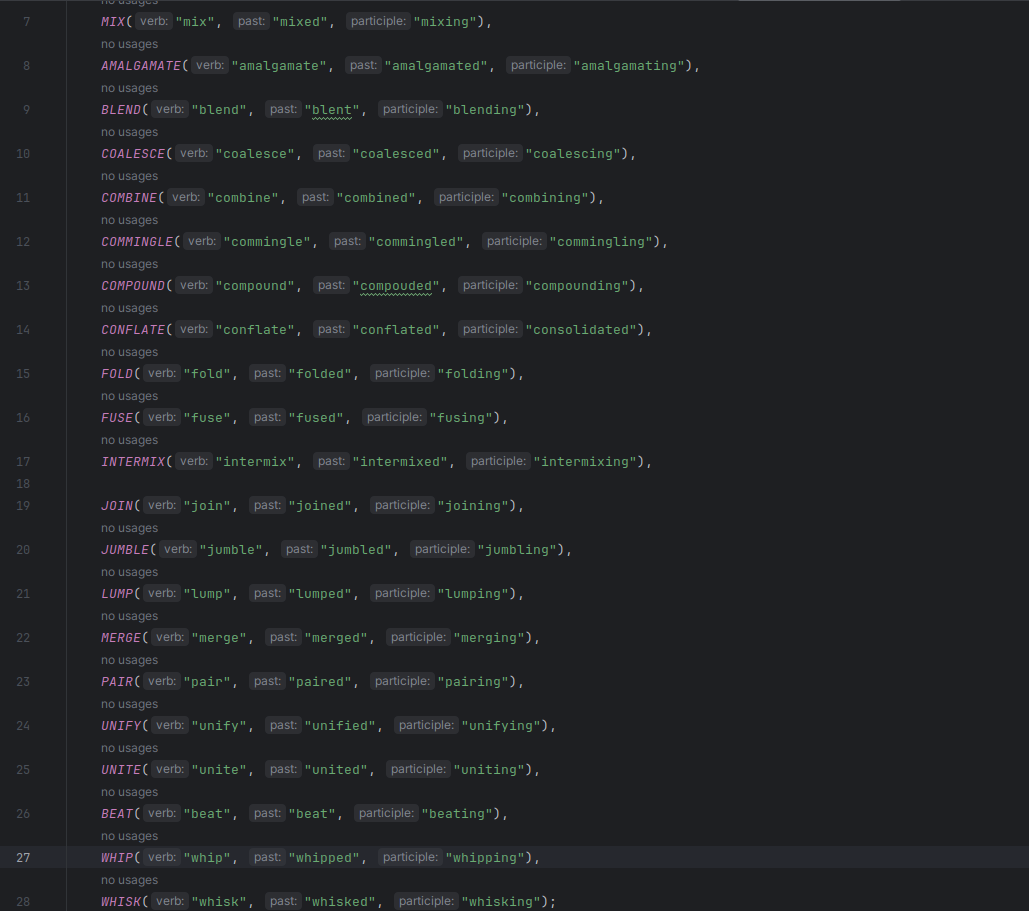
\includegraphics[scale=0.3]{Graphics/MixingVerbClass.png}
    \end{figure}
    IN DEM BILD FEHLT STIRRING
    Since we have now defined the desired verbs that we ultimately want to search for, let's adjust some search parameters. The crucial parameters involve filtering the categories; in our case, we want to focus on mixing in the cooking domain. Therefore, we filter out all articles that do not exist in the Food and Entertaining category.
    \subsubsection*{Hyponyms occurance}
    For each defined verb, a search is initiated to determine how often this verb appears in the WikiHow articles. This is done to ascertain which verbs are ultimately relevant for our implementation and which ones we can exclude, as they are infrequently used in everyday language.
    In the table below the results can be seen.
    \begin{table}[H]
        \centering
        \begin{tabular}{|c|c|}
          \hline
          \textbf{Hyponym} & \textbf{Occurance}  \\
          \hline
          Mix & 5300 \\
          \hline
          Amalgamate & 0 \\
          \hline
          Beat & 956 \\
          \hline
          Blend & 1041 \\
          \hline
          Coalesce & 1 \\
          \hline
          Combining & 3591  \\
          \hline
          Coommingle & 0 \\
          \hline
          Compound & 0 \\
          \hline
          Conflate & 0 \\
          \hline
          Folding & 821 \\
          \hline
          Fuse & 17 \\
          \hline
          Intermix & 0 \\
          \hline
          Join & 53 \\
          \hline
          Jumble & 0 \\
          \hline
          Lump & 7 \\
          \hline
          Merge & 6 \\
          \hline
          Pair & 352 \\
          \hline
          Stir & 6027 \\
          \hline
          Unify & 2 \\
          \hline
          Unite & 2 \\
          \hline
          Whip & 863 \\
          \hline
          Whisk & 2267 \\
          \hline
          
    
        \end{tabular}
        \caption{Mix synoyms/hyponyms occurance}
        \label{tab:example}
      \end{table}
      
  \subsubsection*{Further examination and conclusion}
  This search is ultimately intended to provide us with information on which tasks we want to represent in the knowledge base. Therefore, we decide on certain tasks based on two conditions: frequency and executability. The first condition is easy to understand; tasks that do not occur or occur very rarely are not considered. The second condition relates to the executability of the task in the context of robot movements. Additionally, some tasks with relatively high frequency are also examined more closely, as in English, the past tense is used as an adjective under certain circumstances.

Taking into account the first condition, the following tasks are not considered: Amalgamate, Coalesce, Comingle, Compound, Conflate, Fuse, Intermix, Join, Jumble, Lump, Merge, Unify, and Unite.

The second condition excludes another task: Blend. Blend is mostly used in the context of a blending machine, which is not handled by the robot. Without this machine, the blending execution cannot be performed correctly, so this task is excluded for us.

Upon closer examination, we will also not consider the verb Whip because it is mostly used as an adjective for ingredients, such as whipped cream. This highlights that only the verb Whip has relatively low frequency. The same applies to pair, where the past tense is used to describe a combination of different ingredients, such as wine paired with cheese.

Thus, the tasks we consider are: Mix, Combine, Beat, Fold, Stir, and Whisk.

  \section*{Task analysis and defintion}
  Now that we have selected the tasks, they need to be analyzed to understand the context in which they are ultimately used. Our goal is for the robot to perform these tasks in a manner similar to how a human would. To achieve this, in the next step, we need to closely examine these tasks. It is recommended to analyze videos on WikiHow or other sources where these tasks are presented as activities. The analysis involves observing the movements associated with each task. We present these analyses in tabular form below. The examination includes the task itself, the respective ingredients being processed, the tools used for it, and the container in which the task is carried out.
    \begin{table}[H]
    \centering
    \begin{tabular}{|c|c|c|p{4,5cm}|p{4,5cm}|}
        \hline
        \textbf{Task} & \textbf{Tool} & \textbf{Container} & \textbf{Ingredients} & \textbf{Description} \\
        \hline
        Beating & Whisk & Bowl & Egg yolk (Wet ingredient) & circular, swirling wildly around the bowl \\
        \hline
        Stirring & Whisk & Bowl & Beaten Egg Yolk (Wet), Parmesan(Powder) and Pepper (Powder) & Circular, from the inside to the outside. \\
        \hline
        Stirring & Tongs & Pan & Wet Mixture, Pasta (Solid) and Bacon (Solid) & Diving motions, circular but also straight lines. \\
        \hline
        Whisk & Fork & Bowl & Eggs (Wet) & Circular but also straight, wildly motion. \\
        \hline
        Mixing & Spatula & Pan & Eggs, melted butter (Wet) & Circular, from the inside to the outside, also diving. \\
        \hline
        Folding & Spatula & Pan & cooked eggs in melted butter (Wet) & Gently motion from the outisde to the inside straight, then moving about 90 degree before going to the inside again. \\
        \hline
        Mixing & Spoon & Cup & Dry yeast(Powder), Water (Liquid) & Circular \\
        \hline
        Mixing & Spoon & Bowl & Dry yeast, Water, Flour (Powder), Salt(Powder) & Whirlstorm-like motion. \\
        \hline 
    \end{tabular}
    \caption{Video analysis}
    \label{tab:example}
  \end{table}
NOCH UNVOLLSTÄDNIG

After a thorough analysis of the videos and the information provided in them, we conclude that the executed movement is not only related to the task but also influenced by the ingredients used. However, some tasks are deterministic in the sense that the movement is performed regardless of the specific ingredients.

In the following, we aim to structure the extracted information from the videos and present our findings.

\subsection*{Video analysis conclusion and results}

Based on the extracted information, we conclude that for our goals, the following aspects, in addition to the task, are important and will be further considered:
\begin{itemize}
  \item Ingredients: The ingredients play a crucial role in the movement decision associated with the tasks and will be defined more precisely.
  \item Tools: The tools used may not be decisive in the movement decision, but they are important for the parameters of the robot.????
  \item Container: Das selbe wie oben.
  \item Motions: The motions ultimately represent the movement of the robot for our implementation. These movements are extracted from the videos and defined in alignment with robot motions.
\end{itemize}

\subsubsection*{Ingredients}
Quellen:
\begin{itemize}
  \item https://ceur-ws.org/Vol-2028/paper28.pdf
  \item https://www.freshfarm.org/app/uploads/2020/05/Mixing-Measuring-Wet-and-Dry-Ingredients.pdf
  \item https://www.cookingforengineers.com/article/280/Analyzing-a-Baking-Recipe/print
\end{itemize}
Through the video analysis, we come to the conclusion that the nature of ingredients is important. Primarily, ingredients can be divided into two main categories: Dry and Wet. This division becomes crucial, especially regarding the measurement of quantities for each type of ingredient.

For our case, a somewhat finer categorization of ingredients is necessary to map the various movements sensibly to the given types. In addition to Wet Ingredients, we introduce a new category: Liquid. This corresponds to ingredients falling under Wet Ingredients but with a liquid state, such as milk, water, and oil. This is significant because some movements differ when the given ingredients are Wet or Liquid.

Another category we include is the Solid category. This differs from the Dry category in that it consists of solid components, while we define the Dry category to include powdery substances. The Solid category encompasses foods like vegetables, fruits, and meats. Through these distinctions, we can create a definition refining the ingredient categories.

\textbf{Definition:}
Ingredients are primarily divided into 'Dry' and 'Wet,' with a need for finer differentiation. An abstracted category called 'Liquid' is introduced to encompass liquid states such as milk and water. An additional category, 'Solid,' distinguishes itself from 'Dry' by including solid components like vegetables and meat. These distinctions allow for a precise definition of ingredients, enhancing the analysis of mixing motions in the context of cooking/baking and their representation."
In the initial version, the ingredients we defined are:
\begin{itemize}
  \item Liquid: Milk, Oil, Water, Vinegar, Vanilla Extract, Sauces.
  \item Wet: Egg White, Egg yolk, Butter, Whipped Cream, (mashed fruits?).
  \item Dry: Flour, Salt, Sugar, Baking Soda, Cocoa Powder.
  \item Solid: Onions, Pork, Chicken, Minced meat, Bacon.
\end{itemize}

Hier eventuell nochmal begründen wieso wir die nehmen??.

1. Ansatz: Zutaten aus den Videoanylysen.

2. Ansatz WikiHowExtraction.

\subsubsection*{Tools and Container}
Das kommt von Soma, muss man schauen wie man das beschreiben möchten

\subsubsection*{Motions}
	From this videos we extracted informations about the executed motions. The following motions can be defined:
	\begin{itemize}
		\item \textbf{Circular}: Moving the tool in a defined circular movement in the container, not changing the radius during execution
		\item \textbf{Whirlstorm}: Moving from the inside to the outside of the container with the tool, by circulating in an incremented radius.
		\item \textbf{Folding}: Gently motion, where you start from the outside, moving one straight line to the inner side, then picking the tool up and going to the initial state before moving the tool for about 90 degrees, then going back in a straight line to the inner side of the container again.
		\item \textbf{VerticalCircular}: Imagine a line which can be seen as the diameter of the container, from this line one can define certain regions on which you move the tool circular from side to side. This motion is used by the beating task.
		\item \textbf{CircularDivingToInner}: Starting from the outerside, moving the tool in the container arround its edge for about 270 degrees, before diving to the middle of the container. This motion is used by Tasks where is required to turn the Ingredients over.
	\end{itemize}

\section*{Data Acquision Conclusion}

In the data acquisition phase, our focus was on creating a foundation of the necessary data and information required for a robot to perform various mixing tasks. After identifying the tasks, we were able to analyze videos to examine the movements associated with each task. We concluded that not only the task itself but also the selection of ingredients is crucial for determining the movement.

The ingredients are divided into four different categories, and we were able to define five motions that the robot should perform in a manner consistent with everyday use. In the next chapter, we will present how we intend to represent this knowledge and create a system that enables the robot to know which movement to execute based on a given task and set of ingredients.
\newpage


	\chapter*{Data representation}
	\begin{itemize}
		\item Ingredients, Tools, etc.
		\item Different Tasks/Actions maps on different Motions
		\item Motion dependencies
		\item Fobidden Tools with Containers
		\item How is an action defined
		\item Examples of using the knowledge graph
	\end{itemize}
	\chapter*{Implementation}
	\begin{itemize}
		\item OWLReady
		\item SWRL
		\item Inferring parameters for the actual plan
	\end{itemize}
	\chapter*{Simulation}
	\begin{itemize}
		\item BulletWorld as Simulation platform -> how is the robot actually shown, which limitations exist
		\item Quering the knowledge base
		\item Inferring the parameters in the Simulation
		\item Task execution with multiple sequential Motions
	\end{itemize}
	\section*{Simulation to RealWorld gap}
	\begin{itemize}
		\item Big Problem: Uncertaininty
		\item Perception Solution as first approach: RoboKudo
		\item Data acquisition: Blenderproc
		\item Model Training: YoloV8
		\item Results showing the real world Perception.
	\end{itemize}
	\chapter*{Evaluation}
	\begin{itemize}
		\item Evaluation of multiple motions multiple times
		\item Results of that
	\end{itemize}
	\chapter*{Summary / Fazit}
avc
\end{document}

